\chapter{Further insights from importances}\label{ch:applications}

\begin{remark}{Outline}
In this chapter, we build upon results from Chapter~\ref{ch:importances} to
further study variable importances as computed from random forests. In
Section~\ref{sec:7:redundant}, we first examine importances for variables that
are redundant. In Section~\ref{sec:7:bias}, we revisit variable importances in
the context of binary decision trees and ordered variables. In this framework, we
highlight various sources of bias that may concurrently happen when
importances are computed from actual random forests. Finally, we present in
Section~\ref{sec:7:applications} some successful applications
of variable importance measures.
\end{remark}


\section{Redundant variables}
\label{sec:7:redundant}

In most machine learning problems, it is typical for input variables to be
correlated, at least to some extent, and to share common bits of information.
In image classification for instance, pixels are usually highly correlated and
individually represent nearly the same information as their neighbors. In that
sense, variables are often \textit{partially redundant}, i.e., some of the
variables may share some of the same information about the output variable $Y$.
In the extreme case, redundancy is \textit{total}  or \textit{complete}, with
some of the variables redundantly conveying exactly the same information with
respect to the output variable $Y$. In this section, we study redundancy in
random forests and show that it may have a significant effect on both the
accuracy of the ensemble and variable importance measures.

As a guiding example for our discussion, let us consider a set of input
variables and let us discuss the effect of adding redundant variables on the
structure of randomized trees. Intuitively, two variables $X_i$ and $X_j$ are
redundant if one can perfectly explains the other and vice-versa. Formally, we
define redundancy as follows:

\begin{definition}
Two variables $X_i, X_j$ are totally redundant if the mutual information
$I(X_i;X_j)$ is maximum.
\end{definition}

In particular, a variable $X_j$ and its copy $X_j^\prime$ are totally
redundant. With respect to random forests, adding copies of variables (e.g.,
duplicating $X_j$, hence resulting in a new set of $p+1$ input variables) has
no effect when the selection of the split is deterministic (e.g., in RF for $K$
set to the maximum value). No matter the number of totally redundant variables,
the best split that is selected is always the same, even if the same splits
need to be recomputed multiple times due to redundancy. When the choice of the
best split is stochastic however (e.g., for $K$ strictly smaller than the total number
of variables), adding multiple copies of a variable $X_j$ results in
splits that may be biased towards this variable (or one of its copies), which
in turn may have a significant effect on the resulting accuracy of the
ensemble. For a fixed value of $K$, it is indeed not difficult to see that
adding copies of $X_j$ increases the probability of $X_j$, or of one of its
copies, to be in the random subset of $K$ input variables on which to look for
splits. As a corollary, it therefore also simultaneously decreases the
probability of any of the others to be selected, hence biasing
the structure of resulting decision trees. Note that the resulting net effect
on accuracy depends on the nature of duplicated variable. If $X_j$ is very
informative with respect to the input, then favoring splits on $X_j$ by
adding copies may result in an increase of accuracy. By contrast, if $X_j$
is irrelevant, then adding  copies increases the risk of overfitting.

With respect to variable importances, the effect of adding redundant variables
can be derived both qualitatively and quantitatively using results from
Chapter~\ref{ch:importances}. From Theorem~\ref{thm:relevant}, we already know
that adding irrelevant variables does not change the resulting variable
importances. Adding copies of a relevant variable however, has an effect on
both the importance of the duplicated variable and on the importance of the
remaining variables. As in the previous chapter, let us assume a set $V= \{X_1,
..., X_p\}$  of categorical input variables and a categorical output $Y$, for
which we derive the MDI importance, as computed from totally randomized and
fully developed trees built on an infinitely large dataset.

\begin{lemma}\label{lemma:red1}
Let $X_i$ and $X_j$ be totally redundant variables. For any conditioning set
$B$,
\begin{align}
& I(X_i;Y|B,X_j) = I(X_j;Y|B, X_i) = 0 \label{lemma:red1:eqn1} \\
& I(X_i;Y|B) = I(X_j;Y|B) \label{lemma:red1:eqn2}.
\end{align}
\end{lemma}

\begin{proof}
By definition, if $X_i$ and $X_j$ are totally redundant, then
\begin{equation}
I(X_i;X_j) = H(X_i) - H(X_i|X_j)
\end{equation}
is maximum, which happens when $H(X_i|X_j) = 0$ since $H$ is non-negative.
By symmetry of the mutual information, we similarly have $H(X_j|X_i)=0$,
and therefore $H(X_i)=H(X_j)$. Using the same argument, this directly extends
to any conditioning set $B$, giving:
\begin{align}
& H(X_i|B,X_j) = 0\\
& H(X_j|B,X_i) = 0\\
& H(X_i|B) = H(X_j|B)
\end{align}

From these, it follows that,
\begin{align}
& I(X_i;Y|B,X_j) = H(X_i|B, X_j) - H(X_i|B,X_j,Y) = 0 - 0, \\
& I(X_j;Y|B,X_i) = H(X_j|B, X_i) - H(X_j|B,X_i,Y) = 0 - 0,
\end{align}
which proves Equation~\ref{lemma:red1:eqn1}. We also have
\begin{align}
I(X_i;Y|B) &= H(X_i|B) - H(X_i|B,Y) \\
           &= H(X_j|B) - H(X_j|B,Y) \\
           &= I(X_j;Y|B),
\end{align}
which proves Equation~\ref{lemma:red1:eqn2}.
\end{proof}

\begin{proposition}\label{prop:red:self}
Let $X_j\in V$ be a relevant variable with respect to $Y$ and $V$ and let
$X_j^\prime \notin V$ be a totally redundant variable with respect to $X_j$.
The infinite sample size importance of $X_j$ as computed with an infinite
ensemble of fully developed totally randomized trees built on $V\cup
\{X_j^\prime\}$ is
\begin{equation}
\text{Imp}(X_j) = \sum_{k=0}^{p-1} \frac{p-k}{p+1} \frac{1}{C_p^k} \frac{1}{p-k} \sum_{B \in {\cal P}_k(V^{-j})} I(X_j;Y|B)
\end{equation}
\end{proposition}

\begin{proof}
From Theorem~\ref{thm:imp}, the variable importance of $X_j$ is
\begin{align}
\text{Imp}(X_j) &= \sum_{k=0}^{p-1+1} \frac{1}{C_{p+1}^k} \frac{1}{p+1-k} \sum_{B \in {\cal P}_k(V^{-j} \cup \{X_j^\prime\})} I(X_j;Y|B) \nonumber \\
&= \sum_{k=0}^{p-1} \frac{1}{C_{p+1}^k} \frac{1}{p+1-k} \sum_{B \in {\cal P}_k(V^{-j})} I(X_j;Y|B) \nonumber \\
&= \sum_{k=0}^{p-1} \frac{p-k}{p+1} \frac{1}{C_{p}^k} \frac{1}{p-k} \sum_{B \in {\cal P}_k(V^{-j})} I(X_j;Y|B),
\end{align}
since from Lemma~\ref{lemma:red1}, $I(X_j;Y|B\cup X_j^\prime)=0$ for all $B \in {\cal P}(V^{-j})$.
\end{proof}

\begin{lemma}\label{lemma:red2}
Let $X_i$ and $X_j$ be totally redundant variables. For any conditioning set
$B$ and for any variable $X_l$,
\begin{equation}
I(X_l;Y|B,X_i) = I(X_l;Y|B, X_j) = I(X_l;Y|B, X_i, X_j) \label{lemma:red2:eqn}
\end{equation}
\end{lemma}

\begin{proof}
From the chaining rule of the mutual information, we have
\begin{align}
I(X_i,X_j,X_l;Y|B) &= I(X_l;Y|B) + I(X_i,X_j;Y|B,X_l) \nonumber \\
                   &= I(X_l;Y|B) + I(X_i;Y|B,X_l) + I(X_i;Y|B, X_j, X_l) \nonumber \\
                   &= I(X_l;Y|B) + I(X_i;Y|B,X_l) \quad\text{(Lemma~\ref{lemma:red1})} \nonumber \\
                   &= I(X_i, X_l;Y|B) \nonumber \\
                   &= I(X_i;Y|B) + I(X_l;Y|B,X_i) \label{lemma:red2:eqn1}.
\end{align}
By symmetry,
\begin{equation}\label{lemma:red2:eqn2}
I(X_i,X_j,X_l;Y|B) = I(X_j;Y|B) + I(X_l;Y|B,X_j),
\end{equation}
which proves that $I(X_l;Y|B,X_i) = I(X_l;Y|B, X_j)$, by combining both equations
and using the fact that $I(X_i;Y|B) = I(X_j;Y|B)$ (Lemma~\ref{lemma:red1}).

From the chaining rule, we also have
\begin{align}
I(X_i,X_j,X_l;Y|B) &= I(X_i, X_j;Y|B) + I(X_l;Y|B,X_i,X_j) \nonumber \\
                   &= I(X_i; Y|B) + I(X_j;Y|B, X_i) + I(X_l;Y|B,X_i,X_j) \nonumber \\
                   &= I(X_i; Y|B) + I(X_l;Y|B,X_i,X_j).
\end{align}
By combining this last equation with Equation~\ref{lemma:red2:eqn1},
we finally have $I(X_l;Y|B,X_i) = I(X_l;Y|B,X_i,X_j)$, which proves
Lemma~\ref{lemma:red2}.
\end{proof}

\begin{proposition}\label{prop:red:other}
Let $X_j\in V$ be a relevant variable with respect to $Y$ and $V$ and let
$X_j^\prime \notin V$ be a totally redundant variable with respect to $X_j$.
The infinite sample size importance of $X_l \in V$ as computed with an infinite
ensemble of fully developed totally randomized trees built on $V\cup
\{X_j^\prime\}$ is
\begin{align}\label{prop:red:other:eqn}
\text{Imp}(X_l) &= \sum_{k=0}^{p-2} \frac{p-k}{p+1} \frac{1}{C_p^k} \frac{1}{p-k} \sum_{B \in {\cal P}_k(V^{-l} \setminus X_j)} I(X_l;Y|B) + \\
                & \hookrightarrow \sum_{k=0}^{p-2}  \left[ \sum_{k'=1}^2 \frac{C^{k'}_2}{C_{p+1}^{k+k'}} \frac{1}{p+1-(k+k')} \right]  \sum_{B \in {\cal P}_k(V^{-l}\setminus X_j)} I(X_l;Y|B\cup X_j). \nonumber
\end{align}
\end{proposition}

\begin{proof}
From Lemma~\ref{lemma:red2}, conditioning by either $X_j$, $X_j^\prime$ or by
both  variables yield terms $I(X_l;Y|B,X_j)$, $I(X_l;Y|B,X_j^\prime)$ and
$I(X_l;Y|B,X_j,X_j^\prime)$ that are all equal. From Theorem~\ref{thm:imp}, the
variable importance of $X_l$ can therefore be rewritten as follows:

\begin{align}
\text{Imp}(X_l) &= \sum_{k=0}^{p-1+1} \frac{1}{C_{p+1}^k} \frac{1}{p+1-k} \sum_{B \in {\cal P}_k(V^{-l}\cup X_j^\prime)} I(X_l;Y|B) \nonumber \\
           &= \sum_{k=0}^{p-2} \sum_{k'=0}^2 \frac{1}{C_{p+1}^{k+k'}} \frac{1}{p+1-(k+k')} \sum_{\substack{B \in {\cal P}_k(V^{-l} \setminus X_j)\\ B' \in {\cal P}_{k'}(\{X_j, X_j^\prime\})} } I(X_l;Y|B \cup B') \nonumber \\
           &= \sum_{k=0}^{p-2} \frac{1}{C_{p+1}^k} \frac{1}{p+1-k} \sum_{B \in {\cal P}_k(V^{-l} \setminus X_j)} I(X_l;Y|B) + \nonumber \\
           & \hookrightarrow \sum_{k=0}^{p-2} \left[ \sum_{k'=1}^2 \frac{C^{k'}_2}{C_{p+1}^{k+k'}} \frac{1}{p+1-(k+k')} \right] \sum_{B \in {\cal P}_k(V^{-l} \setminus X_j)} I(X_l;Y|B \cup X_j) \nonumber \\
           &= \sum_{k=0}^{p-2} \frac{p-k}{p+1} \frac{1}{C_p^k} \frac{1}{p-k} \sum_{B \in {\cal P}_k(V^{-l} \setminus X_j)} I(X_l;Y|B) + \nonumber \\
           & \hookrightarrow \sum_{k=0}^{p-2}  \left[ \sum_{k'=1}^2 \frac{C^{k'}_2}{C_{p+1}^{k+k'}} \frac{1}{p+1-(k+k')} \right]  \sum_{B \in {\cal P}_k(V^{-l}\setminus X_j)} I(X_l;Y|B\cup X_j). \nonumber
\end{align}
\end{proof}

Proposition~\ref{prop:red:self} shows that the importance of $X_j$ decreases
when a redundant variable $X_j^\prime$ is added to the set of input variables.
Intuitively, this result is in fact expected since the same information is then
conveyed within two variables (i.e., in $X_j$ and its copy $X_j^\prime$). It
also shows that the terms in the total importance are not all modified in the
same way. The weight of the terms corresponding to small conditioning sets
remains nearly unchanged (i.e., for small values of $k$, $\tfrac{p-k}{p+1}$ is
close to $1$), while the weight of the terms of large conditioning sets is
greatly impacted (i.e., for large values of $k$, $\tfrac{p-k}{p+1}$ tends to
$0$).

As shown by Proposition~\ref{prop:red:other}, the effect of adding a redundant
variable $X_j^\prime$ on the importance of the other variables $X_l$ (for
$l\neq j$) is twofold. The first part of Equation~\ref{prop:red:other:eqn}
shows that the weight of all terms that do not include $X_j$ (or its copy)
strictly decreases by a factor $\tfrac{p-k}{p+1}$. The second part of
Equation~\ref{prop:red:other:eqn} shows that the the weight of all terms that
include $X_j$ (or its copy) increases, since several equivalent conditioning
sets (i.e., $B\cup \{X_j\}$, $B\cup \{X_j\}^\prime$ and $B\cup \{X_j,
X_j^\prime\}$) can now appear within the branches of a tree. Like for
Proposition~\ref{prop:red:self}, impurity terms are not all modified in the
same way and changes depend on the size $k$ of the conditioning set $B$.
Overall, the net effect on the total importance of $X_l$ is therefore a
compromise between these opposing changes. If the weighted sum of the
$I(X_l;Y|B,X_j)$ terms is low with respect to the sum of the terms that do not
include $X_j$ (or its copy), then the decrease effect dominates and the
importance of $X_l$ should be smaller. By contrast, if the $I(X_l;Y|B,X_j)$
terms are larger, then the increase effect dominates and the resulting
importance is larger.

Propositions~\ref{prop:red:self} and \ref{prop:red:other} can be extended to
the case where $N_c$ redundant variables $X_j^c$ (for $c=1,\dots,N_c$) are
added to the input variables instead of one, leading to the general
Proposition~\ref{prop:red:general}. From this result, the same qualitative
conclusions can drawn, except that the decrease or increase effects discussed
above are even stronger as more redundant variables are added.

\begin{proposition}\label{prop:red:general}
Let $X_j\in V$ be a relevant variable with respect to $Y$ and $V$ and let
$X_j^c \notin V$ (for $c=1,\dots,N_c$) be $N_c$ totally redundant variables with respect to $X_j$.
The infinite sample size importances of $X_j$ and $X_l \in V$ as computed with an infinite
ensemble of fully developed totally randomized trees built on $V\cup
\{X_j^1,\dots,X_j^{N_c}\}$ are
\begin{align*}
\text{Imp}(X_j)  &= \sum_{k=0}^{p-1} \left[ \frac{C^k_p (p-k)}{C^k_{p+N_c}(p+N_c-k)}  \right] \frac{1}{C_p^k} \frac{1}{p-k} \sum_{B \in {\cal P}_k(V^{-j})} I(X_j;Y|B), \\
\text{Imp}(X_l) &= \sum_{k=0}^{p-2} \left[ \frac{C^k_p (p-k)}{C^k_{p+N_c}(p+N_c-k)}  \right] \frac{1}{C_p^k} \frac{1}{p-k} \sum_{B \in {\cal P}_k(V^{-l} \setminus X_j)} I(X_l;Y|B) + \\
                & \hookrightarrow \sum_{k=0}^{p-2}  \left[ \sum_{k'=1}^{N_c+1} \frac{C^{k'}_{N_c+1}}{C_{p+N_c}^{k+k'}} \frac{1}{p+N_c-(k+k')} \right]  \sum_{B \in {\cal P}_k(V^{-l}\setminus X_j)} I(X_l;Y|B\cup X_j).
\end{align*}
\end{proposition}

\begin{proof}
Omitted here, but Proposition~\ref{prop:red:general} can be proved
by generalizing for $N_c$ the proofs of Propositions~\ref{prop:red:self}
and \ref{prop:red:other}.
\end{proof}

As an illustrative example, let us reconsider the LED classification problem
from Section~\ref{sec:6:illustration}, and for which $X_5$ was found to be the
most important variable. As shown in Figure~\ref{fig:7:red:led}, adding
variables that are redundant with $X_5$ makes its importance decrease, as
predicted by our theoretical result from Propositions~\ref{prop:red:self} and
\ref{prop:red:general}. When 5 or more copies of $X_5$ are added, the
importance of $X_5$ is the smallest of all, as if $X_5$ had become less
informative. Similarly, we observe that the importance of the other variables
remain about the same or slightly decrease, as if they all had become a bit
less informative. With regards to our previous results in Propositions
\ref{prop:red:other} and \ref{prop:red:general}, this indicates that the
importance due to the $I(X_l;Y|B)$ terms prevails from  the importance due to
the $I(X_l;Y|B,X_5^c)$ terms. As a matter of fact, this example highlights a
fundamental property of variable importances as computed in a random forest:
importance measures are computed not only with respect to the output $Y$, but
also with respect to all the other input variables that define the problem. In
particular, a variable which is not important is not necessarily uninformative,
as the example illustrates. A variable may be considered as less important
because the  information it conveys is also redundantly conveyed in other
variables, and not necessarily because it has no information.

\begin{figure}
\centering
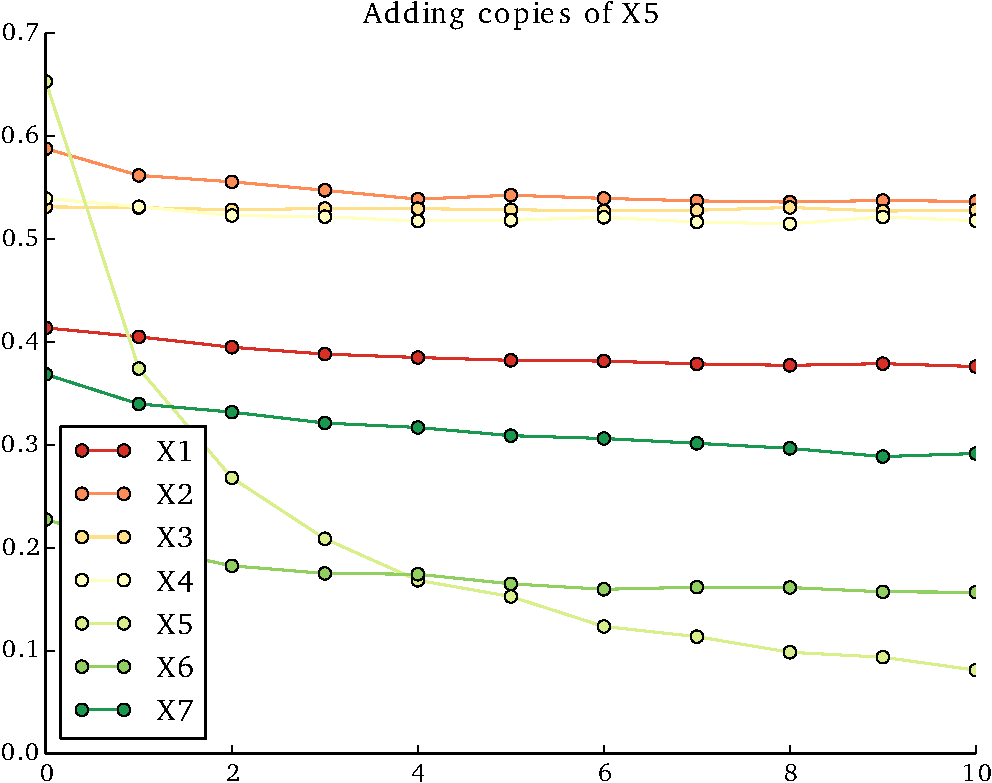
\includegraphics[width=0.9\textwidth]{figures/ch7_red_led.pdf}
\caption{Adding copies of $X_5$ on the LED classification task. The more
         redundant variables are added, the lesser the importance of $X_5$.}
\label{fig:7:red:led}
\end{figure}

As a second example, Figure~\ref{fig:7:red:xor} illustrates redundancy effects
for a XOR classification problem defined on two variables $X_1$ and $X_2$.
Again, the importance of the duplicated variable $X_1$  decreases as redundant
variables are added, which confirms our results from
Propositions~\ref{prop:red:self} and \ref{prop:red:general}. More
interestingly, we now observe that the importance of the other variable, $X_2$,
increases as copies of $X_1$ are added. For this problem, the
$I(X_2;Y|B,X_1^c)$ terms are prevalent with respect to the $I(X_2;Y|B)$ terms
(which is in fact unique and equal to $0$), thereby artificially increasing the
overall importance of $X_2$ as redundancy augments, as expected from
Propositions \ref{prop:red:other} and \ref{prop:red:general}.

\begin{figure}
\centering
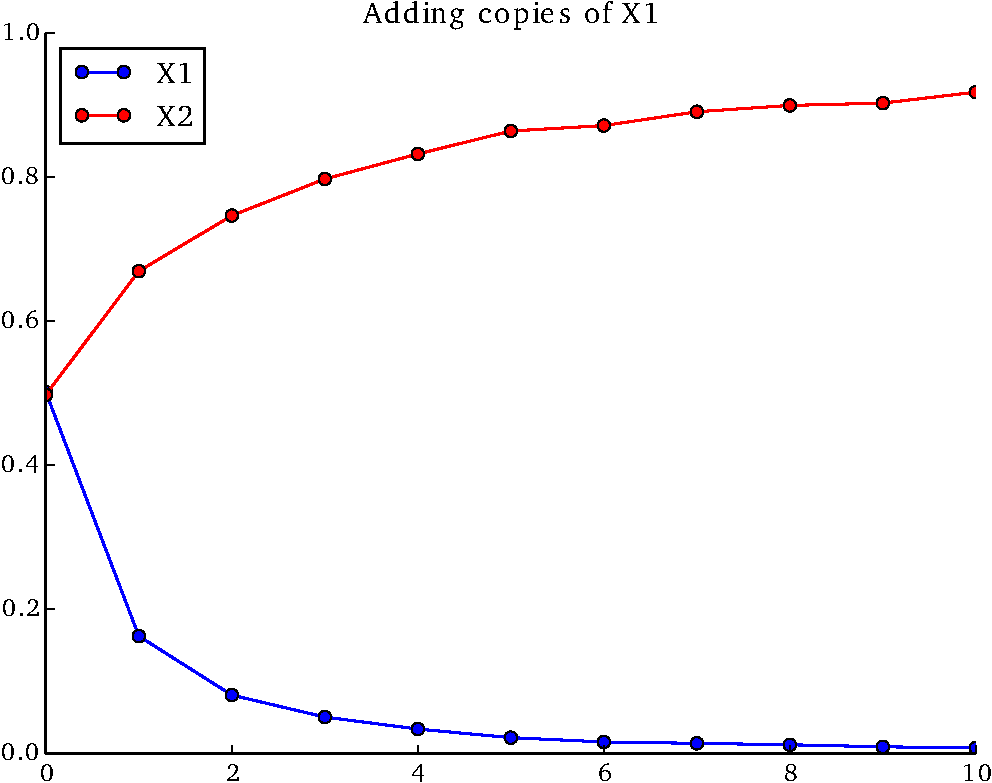
\includegraphics[width=0.9\textwidth]{figures/ch7_red_xor.pdf}
\caption{Adding copies of $X_1$ on a XOR classification task. The more redundant
         variables are added, the lesser the importance of $X_1$, but the larger
         the importance of $X_2$.}
\label{fig:7:red:xor}
\end{figure}

Overall, results presented in this section call for caution when interpreting
variable importance scores. Due to redundancy effects, it may happen that the
total importance of a given variable is either misleadingly low or deceptively
high because the same information is spread within several redundant variables
and therefore taken into account several times within the total importances. As
such, we advise to complement the interpretation with a systematic
decomposition of variable importance scores, e.g., as previously done in
Figure~\ref{fig:decomposition}, in order to better understand why a variable is
in fact important and to possibly detect redundancy.


\section{Bias in variable importances}
\label{sec:7:bias}

In this section, we study sources of bias in variable importances and show that
variable selection (as previously discussed in Section~\ref{sec:ntrt}) is  not
the only cause of bias. In practice, complementary forces due to masking
effects, impurity misestimations and the structure of the trees make variable
importances deviate from the theoretical results found in asymptotic conditions
for totally randomized trees.

\subsection{Bias due to variable selection}

As shown in the previous chapters, the guided selection of the split variable
(i.e., for $K>1$) is necessary for balancing bias and variance in  randomized
decision trees and to produce accurate ensembles. In particular, we studied
that decision trees built with too much randomization usually lead to an
increase of bias which cannot be compensated by a reciprocal decrease of
variance, making it necessary to adjust the value of $K$ to find the
appropriate trade-off. By contrast, we also showed in Section~\ref{sec:ntrt}
that when variable selection is not totally random (i.e., as soon as $K>1$),
masking effects induce a bias with respect to variable importances, since it
forces some of the branches to never be built, and therefore some of the
conditioning sets $B \in {\cal P}(V)$ to never be taken into account. As a
consequence, random forests whose parameter $K$ has been tuned to maximize
accuracy may yield variable importances that are biased. Importances may be
over- or underestimated. More specifically, it can be shown (see
Section~\ref{sec:ntrt}) that a relevant variable may be null with regards to
its importance, thereby making it indistinguishable from irrelevant variables,
and that the importance of relevant variables becomes dependent on the number
of irrelevant variables.

\subsection{Bias due to high cardinality}

To guide our discussion, let us revisit the simulation studies from
\citep{strobl:2007b} which considers a binary output variable $Y$ and five
input variables $X_1,\dots,X_5$, as defined in Table~\ref{table:simulation}.

\begin{table}
    \centering
    \begin{tabular}{| c c c |}
    \hline
    & $X_1$ & $\sim{\cal N}(0, 1)$ \\
    & $X_2$ & $\sim{\cal M}(2)$ \\
    & $X_3$ & $\sim{\cal M}(4)$ \\
    & $X_4$ & $\sim{\cal M}(10)$ \\
    & $X_5$ & $\sim{\cal M}(20)$ \\
    \hline
    \hline
    {\it null case}  & $Y$ & $\sim{\cal B}(0.5)$ \\
    {\it power case} & $Y|X_2=0$ &  $\sim{\cal B}(0.5-\text{relevance})$ \\
                     & $Y|X_2=1$ &  $\sim{\cal B}(0.5+\text{relevance})$ \\
    \hline
    \end{tabular}
    \caption{Input variables are independent random variables as defined from
    the table. ${\cal N}(0, 1)$ is the standard normal
    distribution. ${\cal M}(k)$ is the multinomial distribution with values in $\{0, \dots, k-1\}$
    and equal probabilities. ${\cal B}(p)$ is the binomial distribution. In the
    null case, $Y$ is independent from $X_1, \dots, X_5$. In the power case, $Y$
    depends on the value $X_2$ while other input variables remain irrelevant.}
    \label{table:simulation}
\end{table}

\begin{figure}
\centering
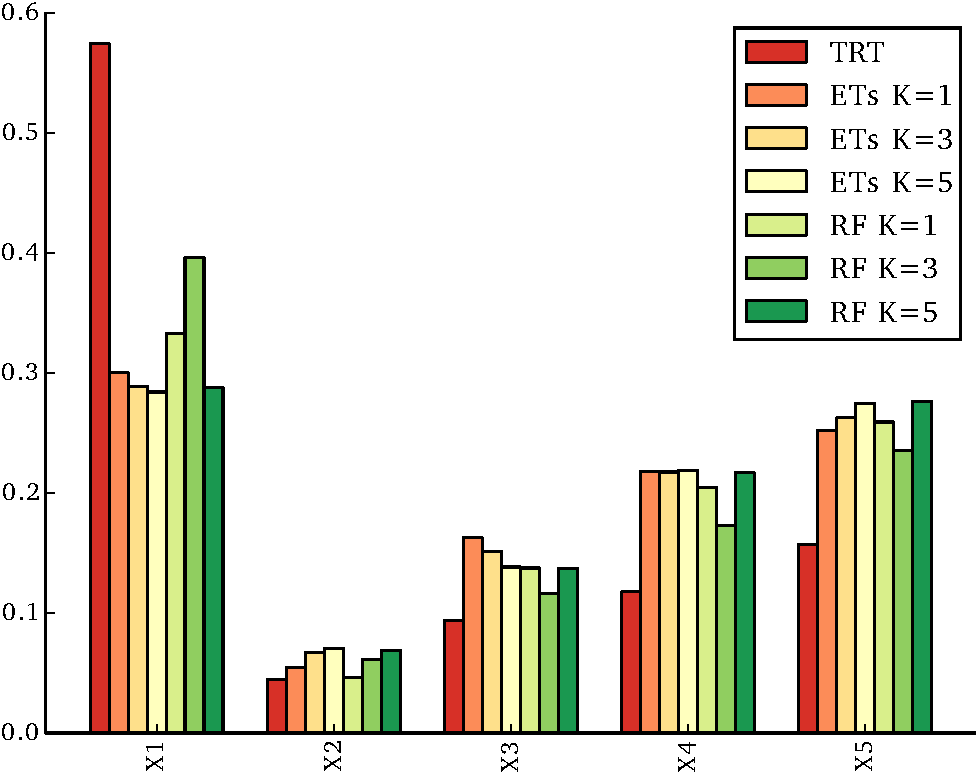
\includegraphics[width=0.9\textwidth]{figures/ch7_bias_null.pdf}
\caption{Variable importances for $Y$ independent of $X_1, \dots, X_5$. ($N=120$, $M=500$)}
\label{fig:7:bias:null}
\end{figure}

Let us first analyze the case where $Y$ is independent from $X_1, \dots, X_5$,
i.e., such that none of the input variables are informative with respect to the
output. For a randomly sampled dataset ${\cal L}$ of $N=120$ samples,
Figure~\ref{fig:7:bias:null} plots variable importances for different kinds of
random forests. ID3 corresponds to multiway totally randomized trees, as
defined in Section~\ref{sec:6:theory}, RF corresponds to Random Forest with
bootstrap sampling and ETs corresponds to Extremely Randomized Trees. In
asymptotic conditions, we proved in Theorem~\ref{thm:irrelevant} that the
importance of irrelevant variables is strictly equal to $0$. For a finite value
of $N$ however, this result does not hold, as Figure~\ref{fig:7:bias:null}
indeed confirms. In contrast with what would be expected, we observe that the
importance of none of the variables is in fact close to $0$. More importantly,
we also observe that the larger the cardinality of the variable (i.e., the
larger its number of unique values), the larger its importance. For example,
the importance of $X_1$ (for which samples all have unique values) or of $X_5$
(which counts up to $40$ unique values) appears nearly $3$ times larger as the
importance of $X_2$ (which is binary).

In their study, \citet{strobl:2007b} argue that this bias is due to variable
selection: \textit{variables with more potential cut-points are more likely to
produce a good criterion value by chance, as in a multiple testing situation}.
As a result, variables of higher cardinality are more likely to be chosen for
splitting than those of lower cardinality. While this bias has been known for
long in decision trees~\citep{kononenko:1995,kim:2001,hothorn:2006}, we argue
that it is not the actual cause for the bias observed here. Indeed, this
argument does not directly explain why similar trends are also observed when no
variable selection is performed (e.g., for ID3 or for $K=1$) nor why it
similarly happens when cut-points are chosen at random, independently of the
cardinality of the variable (e.g., in ETs).

For multiway splits like in ID3, bias in variable importances can be traced to the
misestimations of the mutual information terms
\begin{equation}
\Delta i(s, t) \approx I(X_j;Y|t)
\end{equation}
due to the finite size $N_t$ of the node samples. As shown in
\citep{goebel:2005}, when $X_j$ and $Y$ are independent random variables (i.e.,
when $X_j$ is irrelevant), the distribution of finite sample size estimates of
their mutual information  follows approximately a gamma distribution whose mean
is linearly proportional to the cardinalities $|{\cal X}_j|$ and $|{\cal Y}|$
of $X_j$ and $Y$ and inversely proportional to $N_t$.
As a result, estimates get larger as $X_j$ counts many unique values, and
become even larger as nodes are deep in the tree (since $N_t$ gets smaller).
Consequently, the weighted mean of all such estimated impurity terms
$I(X_j;Y|t)$, for all nodes $t$ where $X_j$ is the split variable, and
resulting in the total importance $\text{Imp}(X_j)$, is also linearly dependent
on the cardinality of $X_j$. For ID3, this result explains why variables of
high cardinality in Figure~\ref{fig:7:bias:null} appear as more important than
those of lower cardinality. Intuitively, the closer the number of unique values
with respect to the total number of samples, the larger the impurity decrease
when splitting exhaustively on this variable. In the extreme case, when values
for $X_j$ are all unique, splitting on the variable perfectly memorizes the
values of $Y$, resulting in child nodes that are all pure, therefore maximizing
the estimated mutual information. As such, this explains why $X_1$, whose
values are all unique, appears as the most important variable.

For binary splits (i.e., for RF and ETs, but not for ID3) the mutual
information $I(X_j;Y|t)$ is not directly estimated at each node. Rather, in the
case of ordered variables, $\Delta i(s, t)$ corresponds to an estimate of the
mutual information $I(X_j\leq v;Y|t)$ of the binary split $X_j \leq v$. Under
the simplifying assumption that binary splits on the same variable are all
directly consecutive in the decision tree,  it is easy to see that recursive
binary partitioning eventually ends up emulating direct multiway exhaustive
splits. Using an argument similar to the proof of Theorem~\ref{thm:sum-of-imp},
intermediate impurity terms between the first split and the last of those
splits cancel each other when summing up the importances, which finally amounts
to collect an actual estimate of $I(X_j;Y|t)$ from the binary splits. For the
same reasons as before, variables of high cardinality are therefore biased in
the same way. (As we will study in Section~\ref{sec:bias:tree}, this assumption
does not hold in practice, making the importances from binary decision trees
strictly different from those of multiway decision trees. Yet, the qualitative
conclusions are still valid since variables of high cardinality can be reused
far more many times within the same tree than variables of low cardinality.)

In both situations, the origin of the problem stems from the fact that node
impurity is misestimated when the size $N_t$ of the node samples is too small.
To a large extent, the issue is aggravated by the fact that trees are fully
developed by default, making impurity terms collected near the leaves usually
unreliable. As a precaution, a safe and effective solution for the bias problem
therefore simply consists in collecting impurity terms only for those nodes
where the impurity estimates can be considered as reliable. Equivalently, the
construction of the tree can also be stopped early, when impurity estimates
become unreliable, e.g., using one of the stopping criteria defined in
Section~\ref{sec:3:stop}. Among all alternatives, conditional inference
trees~\citep{hothorn:2006} make use of statistical tests for assessing the
independence of $X_j$ and $Y$ at a pre-specified level of confidence $\alpha$.
If the null hypothesis cannot be rejected, then recursive partitioning halts.
In particular, variable importances collected from such trees were shown
experimentally by \citet{strobl:2007b} not to suffer from bias. The authors
argue that it is due the unbiased variable selection mechanisms also
implemented in conditional inference trees. By contrast, we argue that, by and
large, the absence of bias in importances from such trees is mostly due to the
early stopping criterion, and not to variable selection.

\begin{figure}
\centering
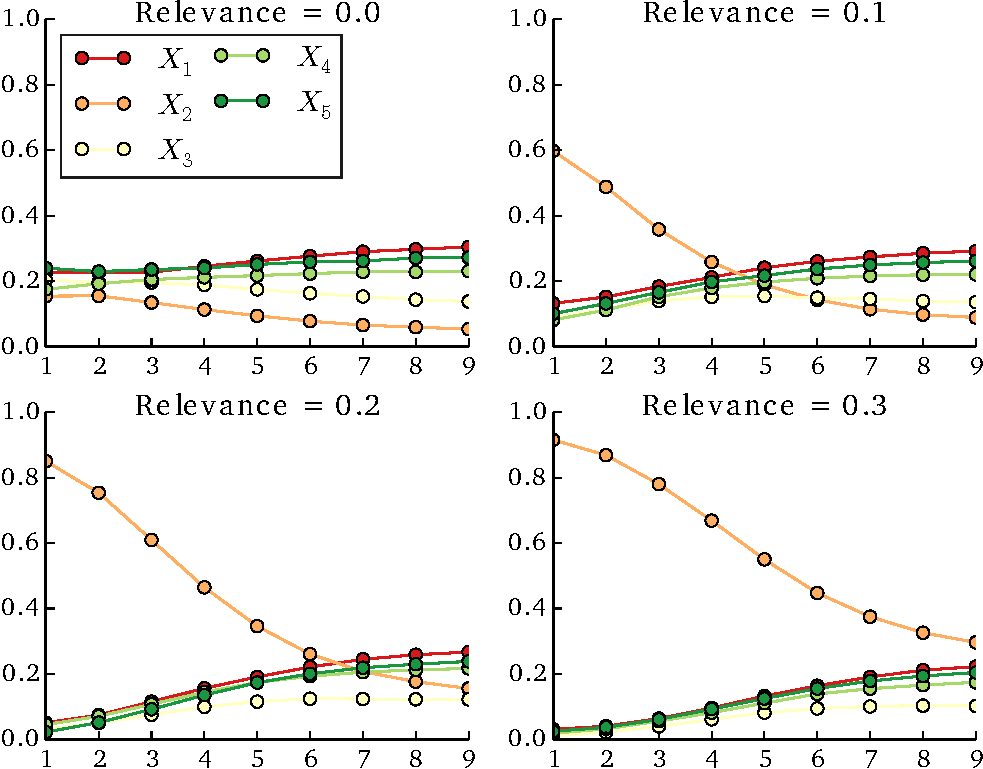
\includegraphics[width=0.9\textwidth]{figures/ch7_bias_depth.pdf}
\caption{Variable importances of $X_1, \dots, X_5$ when varying both the
    maximum depth of trees and the degree of relevance of $X_2$. (ETs, $K=1$, $N=120$, $M=500$)}
\label{fig:7:bias:depth}
\end{figure}

As an illustrative example, Figure~\ref{fig:7:bias:depth} reconsiders the
simulation study of Table~\ref{table:simulation} for ETs  built with no
variable selection ($K=1$), when varying both the maximum depth of trees (from
$\texttt{max\_depth}=1$ to $9$) and the relevance of $X_2$ with respect to
$Y$.


% agravé ar des arbres totalement développés
% early stop to have good estimations


% I est misestimé
% - car on a pas assez d'échantillons par noeud
% - agravé par le fait qu'on développe totalement les arbres
% - conséquence pour celle de grande cardinalité \citep{goebel:2005}

% on peut exhauster plus vite


% * bias due to masking effects, caused by the variable selection (K>1)
%   S: K=1
%
% * bias towards high cardinality, for irrelevant variables
%   - this seems logical when K>1 (page14+ strobl, masking effects due to selection)
%   - but why is this still true for K=1?
%   - montrer par un exemple (e.g., reproduire strobl)
%   - montrer cependant que l'effet s'atténue à mesure que N augmente (choisir une méthode, fixer max_depth avec ou sans)
%       * pour chaque valeur de X, on finit par retrouver toutes les valeurs de y)
%   - et/ou en limitant la profondeur
%   => due to a misestimation of  I(X;Y)
%      noter que l'erreur est d'autant grande plus qu'on splitte de façon exhaustive
%   => Effet du à la misestimation de I(X;Y) en raison d'un nombre trop peu important de samples
%      condition à la consistence: faire en sorte que les feuilles grandissent moins vite que N
%       e.g. fixer max_depth ou min_samples_leaf
%   S: limiter la profondeur
%   S: exhaustive splits
%   S: characterize in a finite setting

\subsection{Bias due to the tree structure}
\label{sec:bias:tree}

% * bias due to the conditioning sets that are evaluated
%   - splitting in binary trees on non-binary variables is like having
%     several binary variables, and to adjust the probability of selecting them
%   - a branch may comprise several values for b (i.e. B<=b plutot que B=b)
%     trouver un exemple qui montre que ça biaise
%   S: exhaustive splits => seulement si N large, splits intermédiaires
%

\subsection{Bias due to threshold selection}

% * bias due to masking effects, caused by the selection of the thresholds
%   - c'est commme si on on n'utilisait jamais certaines variables de l'encodage binaire
%   - bias may be positive or negative (eg, for ETs)
%   - ~= biais du à la discrétization => ID3 n'en souffre pas
%   S: exhaustive splits
%
% * est-ce que la non-equiprobabilité des arbres est une source de biais?
%   - étudier la fréquence des conditionnements pour s'en assurer
%
% Solutions:
% - ID3-like are not biased in that sense
%
% Related work

% ---
% piste de recherche: approximer splits exhaustifs par des splits limités à n branches max
% bonus: pour n=2, on retrouverait le cas binaire
% quelle est l'erreur d'approximer?
% comment former les paquets à mettre dans chaque branche?


\section{Applications}
\label{sec:7:applications}

% Explain Vincent paper
% reproduire experience de microarray dans "Manual on setting up, using, and understanding random forests v3. 1/v4"
